% Template for Cogsci submission with R Markdown

% Stuff changed from original Markdown PLOS Template
\documentclass[10pt, letterpaper]{article}

\usepackage{cogsci}
\usepackage{pslatex}
\usepackage{float}
\usepackage{caption}

% amsmath package, useful for mathematical formulas
\usepackage{amsmath}

% amssymb package, useful for mathematical symbols
\usepackage{amssymb}

% hyperref package, useful for hyperlinks
\usepackage{hyperref}

% graphicx package, useful for including eps and pdf graphics
% include graphics with the command \includegraphics
\usepackage{graphicx}

% Sweave(-like)
\usepackage{fancyvrb}
\DefineVerbatimEnvironment{Sinput}{Verbatim}{fontshape=sl}
\DefineVerbatimEnvironment{Soutput}{Verbatim}{}
\DefineVerbatimEnvironment{Scode}{Verbatim}{fontshape=sl}
\newenvironment{Schunk}{}{}
\DefineVerbatimEnvironment{Code}{Verbatim}{}
\DefineVerbatimEnvironment{CodeInput}{Verbatim}{fontshape=sl}
\DefineVerbatimEnvironment{CodeOutput}{Verbatim}{}
\newenvironment{CodeChunk}{}{}

% cite package, to clean up citations in the main text. Do not remove.
\usepackage{apacite}

% KM added 1/4/18 to allow control of blind submission


\usepackage{color}

% Use doublespacing - comment out for single spacing
%\usepackage{setspace}
%\doublespacing


% % Text layout
% \topmargin 0.0cm
% \oddsidemargin 0.5cm
% \evensidemargin 0.5cm
% \textwidth 16cm
% \textheight 21cm

\title{Individual differences in habituation rate and behavioral
volatility predict dishabituation in adults, preschoolers and infants}

\usepackage{booktabs} \usepackage{graphicx} \usepackage{makecell}

\author{{\large \bf Morton Ann Gernsbacher (MAG@Macc.Wisc.Edu)} \\ Department of Psychology, 1202 W. Johnson Street \\ Madison, WI 53706 USA \AND {\large \bf Sharon J.~Derry (SDJ@Macc.Wisc.Edu)} \\ Department of Educational Psychology, 1025 W. Johnson Street \\ Madison, WI 53706 USA}

\newlength{\cslhangindent}
\setlength{\cslhangindent}{1.5em}
\newenvironment{CSLReferences}%
  {}%
  {\par}

\begin{document}

\maketitle

\begin{abstract}
From infancy to adulthood, habituation and dishabituation enable
learners to filter out repetitive information and remain attentive to
novelty. Here, we leveraged large-scale datasets spanning infants,
preschoolers, and adults to examine how individual differences in
habituation parameters (e.g., decay rate, attention variability) predict
dishabituation. We found that faster habituation consistently related to
stronger attention recovery to novel stimuli. In addition, higher
variability in looking behavior during repeated stimulus exposures
predicted greater dishabituation in adults. We also observed that
different measures of dishabituation yielded somewhat divergent
patterns, highlighting the importance of robustness checks on
exploratory analysis. These findings reveal how endogenous factors are
meaningful drivers of looking behaviors. Overall, our results underscore
the need for large-scale data approaches to studying visual attention
across the lifespan.

\textbf{Keywords:}
habituation; looking time; mega-analysis; individual differences
\end{abstract}

Habituation and dishabituation are fundamental processes in learning and
cognition. Habituation refers to the decrease in response to a repeated
stimulus, while dishabituation describes the renewed increase in
response following the introduction of a novel stimulus. These processes
are essential for learning from experience and have been widely
documented across a broad range of species (Rankin et al., 2009;
Thompson, 2009). From single-cell organisms (e.g., Boisseau, Vogel, \&
Dussutour, 2016; Dussutour, 2021; Ginsburg \& Jablonka, 2009) to humans
{[}e.g. Colombo \& Mitchell (2009); Jeffrey \& Cohen (1971); Sokolov
(1990);{]}, habituation and dishabituation enable individuals to filter
out repetitive, non-informative stimuli while remaining sensitive to
novel or meaningful changes. These mechanisms have become a cornerstone
of research methods in cognitive development (Aslin, 2007; Cohen, 2004;
Kucharskỳ, Zaharieva, Raijmakers, \& Visser, 2024; Oakes, 2010). A
typical infant study utilizing the habituation paradigm involves
repeatedly presenting an infant with the same stimulus until they
exhibit a decline in interest, often measured by a progressive decrease
in looking time. Once habituation is established (e.g., looking time in
the final trials must drop to 50\% of initial looking), the infant is
presented with two stimuli: one familiar (previously shown) and one
novel. A dishabituation response---indicated by significantly longer
looking time at the novel stimulus---suggests that the infant can
discriminate between the two. Dishabituation magnitude serves as a
crucial index of attentional recovery and sensitivity to novel stimuli.
In this work, we used existing data collected using this method to study
individual differences in dishabituation, and what individual-level
predictors (e.g.~habituation rate and age) and experiment-level
predictors (e.g.~stimulus complexity) account for those differences.

\hypertarget{endogenous-and-exogenous-factors-driving-looking-behavior}{%
\subsubsection{Endogenous and exogenous factors driving looking
behavior}\label{endogenous-and-exogenous-factors-driving-looking-behavior}}

Understanding how endogenous and exogenous factors-- differences between
individuals and differences between tasks-- interact to guide looking
behavior is crucial for developing a comprehensive model of early
learning. In one influential model of habituation (Hunter \& Ames,
1988), learners, including infant learners, engage with stimuli to
optimize learning. This leads to the predictions that (i) more efficient
learners (e.g.~older infants) should habituate faster than less
efficient learners (e.g.~younger infants), (ii) learners should recover
attention to novel stimuli as they become more habituated with familiar
stimuli, and (iii) learners should engage with a stimulus relative to
its information value. All of these predictions have enjoyed empirical
support (Cao, Raz, Saxe, \& Frank, 2023; Kidd, Piantadosi, \& Aslin,
2012; Raz, Cao, Saxe, \& Frank, 2025). Particularly striking are studies
of individual differences, suggesting that some differences could serve
cognitive markers with long-term implications. Habituation rate---how
quickly an infant's attention declines in response to repeated exposure
to a stimulus---has been associated with foundational cognitive
processes such as information processing speed (Hunter \& Ames, 1988;
Poli et al., 2024). Infants who habituate more quickly tend to show
higher IQ scores, better language acquisition, and stronger executive
function abilities in later childhood (Colombo, Shaddy, Richman,
Maikranz, \& Blaga, 2004; Kavšek, 2004; Slater, 1997). Similarly,
individual differences in dishabituation---the extent to which an
infant's attention recovers when presented with a novel stimulus---have
been associated with stronger recognition memory (Fagan III, 1984; Fagan
\& Singer, 1983).

Another striking example comes from studies manipulating environmental
volatility, or the predictability of upcoming stimuli. Poli et al.
(2024) demonstrated that infant learners adjust their looking behavior
in response to volatility: they initiate saccades more quickly when
stimuli are highly unpredictable. Yet, we know less about whether
volatility varies as a function of the learners, as well as the learning
context. On the one hand, behavioral variability has often been
interpreted as random noise (Faisal, Selen, \& Wolpert, 2008; Renart \&
Machens, 2014) or a lack of control (Todorov, 2004). In the context of
habituation and dishabituation, these accounts would predict that
greater behavioral volatility during habituation would be unrelated to
subsequent dishabituation, or predict weaker dishabituation. On the
other hand, behavioral volatility could also be adaptive, reflecting an
enhanced sensitivity to potential environmental contingencies and more
dynamic attention regulation (Aston-Jones \& Cohen, 2005; Wu, Miyamoto,
Castro, Ölveczky, \& Smith, 2014). In the context of habituation and
dishabituation, higher volatility in looking time may indicate greater
flexibility in attention allocation, potentially leading to greater
dishabituation by allowing learners to remain more responsive to novel
stimuli.

\hypertarget{the-challenge-of-studying-drivers-of-looking-behavior}{%
\subsubsection{The challenge of studying drivers of looking
behavior}\label{the-challenge-of-studying-drivers-of-looking-behavior}}

Systematically studying how different endogenous and exogenous factors
shape looking time in the habituation paradigm---especially across
different age groups and stimulus contexts---remains challenging.
Recruiting and testing large infant samples can be highly
resource-intensive (DeBolt, Rhemtulla, \& Oakes, 2020; Oakes, 2017),
making it difficult to capture sufficient variability. Additionally,
habituation outcomes can be influenced by measurement noise and fixed
threshold criteria (Dannemiller, 1984; Kucharskỳ et al., 2024; Thomas \&
Gilmore, 2004), which risk misclassifying infants' true levels of
attention. As a result, genuine variability in cognitive processing may
be obscured by methodological artifacts. To overcome these limitations
and capture more reliable estimates of individual differences,
researchers have increasingly adopted large-scale data approaches such
as meta-analysis and mega-analysis (Bergmann et al., 2018; Koile \&
Cristia, 2021), as well as online studies, which facilitate the
recruitment of large and diverse participant samples (Chuey et al.,
2021; Chuey, Boyce, Cao, \& Frank, 2024; Sheskin et al., 2020).

Here, we use large-scale datasets from online studies and mega-analysis
to explore how individual differences in habituation rate predict
dishabituation magnitude. Unlike previous work focused solely on infancy
(Gilmore \& Thomas, 2002; Šimkovic \& Träuble, 2021; cf Cao et al.,
2023; Raz et al., 2025), here we take a lifespan approach, examining
habituation and dishabituation from infancy to adulthood. In addition,
we also explored how dishabituation was shaped by factors like
habituation volatility (e.g., fluctuations in looking time), age, and
stimulus complexity shape dishabituation. By comparing across three age
groups, we provide new insights into developmental continuity and
discontinuity. To preview our findings, we found (1) Individuals who
habituate faster show a stronger rebound in attention to novel stimuli;
(2) In adults, but not younger participants, greater variability in
looking time during habituation is associated with stronger
dishabituation, and (3) Different operationalizations of dishabituation
yield somewhat divergent results.

\hypertarget{methods}{%
\section{Methods}\label{methods}}

\captionsetup{belowskip=0pt,aboveskip=0pt}

\begin{CodeChunk}
\begin{figure*}[h]

{\centering 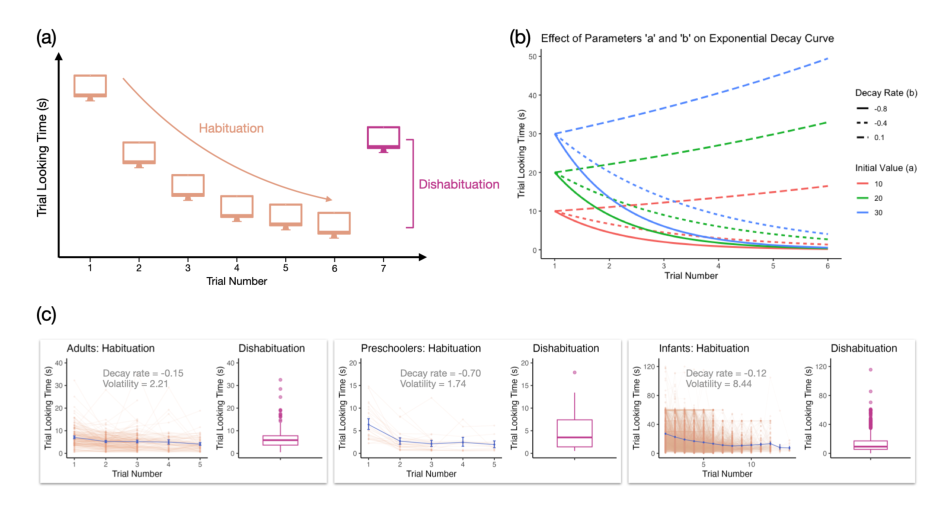
\includegraphics{figs/experimental_design-1} 

}

\caption[(a)Conceptual diagram illustrating habituation (looking times decrease with repeated exposures to the same stimulus) and subsequent dishabituation (a renewed increase in looking time when a novel stimulus is presented).(b) Exponential decay curves showing how variation in the initial value ($a$) and decay rate ($b$) affects the slope and starting point of the habituation trajectory]{(a)Conceptual diagram illustrating habituation (looking times decrease with repeated exposures to the same stimulus) and subsequent dishabituation (a renewed increase in looking time when a novel stimulus is presented).(b) Exponential decay curves showing how variation in the initial value ($a$) and decay rate ($b$) affects the slope and starting point of the habituation trajectory. More negative $b$ values reflect faster declines in looking time.(c) Empirical examples of habituation (left) and dishabituation (right) across adults, preschoolers, and infants. Each panel shows mean trajectories (lines), individual participant trajectories (light lines), and the corresponding boxplot of dishabituation. The group average decay rate and volatility (the standard deviation of residuals) are noted below each age group’s plot, illustrating differences in habituation and dishabituation across the lifespan.}\label{fig:experimental_design}
\end{figure*}
\end{CodeChunk}

\hypertarget{datatasets}{%
\subsection{Datatasets}\label{datatasets}}

We used three datasets, each measuring habituation and dishabituation in
adults (Cao et al., 2023), preschoolers (Raz, Cao, Bui, Frank, \& Saxe,
2023), and infants (Kunin, Piccolo, Saxe, \& Liu, 2024).

\hypertarget{adults}{%
\paragraph{Adults}\label{adults}}

The adult dataset was collected using a web-based, self-paced looking
time paradigm. In this experiment, participants were presented with a
sequence of animated creatures and could advance to the next trial at
their own pace by pressing the down arrow key. Each block consisted of
six trials, with one repeating stimulus and one deviant stimulus. The
deviant stimulus appeared at either the second, fourth, or sixth trial
of the block. Since the current analysis focuses on habituation
trajectories, we preprocessed the data to ensure that the deviant
stimulus only appeared in the fourth or sixth trial and included only
the first block for each participant to prevent across-block habituation
effects. The final dataset consists of 186 habituation-dishabituation
sequences from 186 English-speaking participants recruited through
Prolific (Age: \(M\) = 28.98 Years, \(SD\) = 9.32 Years; 111 F; 72 M; 2
NA).

\hypertarget{preschoolers}{%
\paragraph{Preschoolers}\label{preschoolers}}

The design of the preschooler study was similar to the adult study, with
the key difference that it was administered in person at a
university-affiliated preschool in the United States using a laptop. We
applied the same preprocessing steps as in the adult dataset to maintain
consistency. The final dataset includes 33 habituation-dishabituation
sequences from 33 participants (Age: \(M\) = 54.5 Months, \(SD\) = 8.35
Months). We note that this dataset is substantially smaller than the two
others, and thus will interpret the results with caution.

\hypertarget{infants}{%
\paragraph{Infants}\label{infants}}

The infant dataset was compiled through a systematic literature review
and meta-analytic approach, drawing from studies that examined infants'
habituation and dishabituation responses in violation-of-expectation
(VOE) paradigms. The dataset includes infant-level data from studies
published after 1985 that tested typically developing infants between 3
and 12 months of age on expectations about physical objects or agents
engaging in intentional actions. A typical paradigm involves two phases:
in the habituation phase, infants are presented with a sequence of
repeating stimulus. In the test phase, infants are presented with a
stimulus that is either perceptually novel but conceptually similar to
the repeating stimulus, or conceptually novel but perceptually similar.
The current analysis focuses on perceptual dishabituation -- that is,
comparing test trials with perceptually novel stimuli to the last
dishabituation trial. To ensure data quality, we excluded participants
with fewer than three habituation trials. The final dataset includes
1986 habituation-dishabituation sequences from 1986 participants (Age:
\(M\) = 224.9 Days, \(SD\) = 96.45 Days; 1004 F; 955 M; 27 NA).

\hypertarget{analytic-approach}{%
\subsection{Analytic approach}\label{analytic-approach}}

All analyses were conducted in R using the nlme package (Pinheiro et
al., 2017). All data and analysis scripts can be accessed from XXX.
These analyses were exploratory, but we provided a robustness check in
section Robustness Check

\hypertarget{selecting-exponential-decay-parameters-for-each-age-group.}{%
\paragraph{Selecting exponential decay parameters for each age
group.}\label{selecting-exponential-decay-parameters-for-each-age-group.}}

We follow the conventions of a vast prior literature (Ashmead \& Davis,
1996; Dannemiller, 1984; Sirois \& Mareschal, 2002; Thompson \& Spencer,
1966) and model habituation with an exponential decay. Here, we fit a
nonlinear mixed-effects (NLME) model with an exponential decay function
on each dataset. The function takes the general form of:
\texttt{LT\ \textasciitilde{}\ a\ *\ exp(b\ *\ trial\_number)}. The
parameter a is the intercept, representing initial looking time, and b
is the decay rate, reflecting the speed of habituation (See FIGURE 1 for
schematic illustration of how a and b shapes the habituation
trajectory).

First, we used a data-driven approach to ask, for each age group, which
parameters explain variability in habituation across individuals (and
thus, which parameters are worth studying as predictors of
dishabituation).We selected the model with the lowest Akaike Information
Criterion (AIC), with a \(\Delta_{AIC} > 4\) suggesting substantial
support for the model with lower AIC (Burnham \& Anderson, 2004), among
the models with the following random effects:

\begin{enumerate}
\def\labelenumi{\arabic{enumi}.}
\item
  Random effects on \(a\) only -- allows individual variation in initial
  looking time but assumes a shared decay rate across participants.
\item
  Random effects on \(b\) only -- allows individual variation in decay
  rate while assuming a common initial looking time across participants.
\item
  Random effects on both \(a\) and \(b\) -- allows individual variation
  in both parameters (Note: In the model, we explicitly assumed a and b
  are uncorrelated because they are conceptually independent. Moreover,
  this constraint improves statistical parsimony by reducing model
  complexity.)
\end{enumerate}

\hypertarget{additional-predictors.}{%
\paragraph{Additional predictors.}\label{additional-predictors.}}

In addition to parameters related to exponential decay, we examined
three additional predictors: volatility (how much looking behavior
varied over the course of habituation), stimulus complexity (whether the
stimuli participants saw were relatively simple or complex), and
participant age. Volatility was defined as the standard deviation of the
model residuals across habituation trials for each age group, capturing
the extent to which looking behavior fluctuates over time (Li, Liu,
Hartman, \& Belsky, 2018; Li, Sturge-Apple, Platts, \& Davies, 2023). In
the adult datasets, complexity was explicitly manipulated (throughout
the experiment, participants saw creatures that had more body parts, or
fewer). In the infant dataset, complexity was defined by the domain of
the stimuli (studies involving agents acting on objects were deemed more
complex than studies involving only inanimate objects). The preschooler
dataset did not include complexity information. Participant age was
available for all datasets, and we converted the original units in each
dataset to months to facilitate better comparison. Finally, since the
infant dataset has sufficient variation to estimate initial looking time
for each individual, we include it as a predictor as well.

\hypertarget{selecting-measures-of-dishabituation.}{%
\paragraph{Selecting measures of
dishabituation.}\label{selecting-measures-of-dishabituation.}}

Our main behavior of interest -- recovering attention to a novel
stimulus, after seeing a series of repeated stimuli -- is best captured
as a contrast between looking at the novel stimulus and looking at the
prior (familiar) stimulus, right before the novel stimulus is shown. But
one challenge in selecting a measure of dishabituation is to ensure that
it is de-confounded from individual differences in participants' overall
tendency to look at stimuli. Thus, we took two approaches to measure
this contrast.

The first was a residual-based approach. Residual is the difference
between an observed value and the predicted value from a model. We
calculated the dishabituation magnitude as the following:

\(Dishabituation = r_{dishab} - r_{lasthab}\)

\(r_{dishab}\) was extracted from fitting an intercept-only linear model
on all dishabituation trials:
\texttt{LT\ \textasciitilde{}\ lme(trial\_looking\_time\ \textasciitilde{}\ 1,\ \ random\ =\ \textasciitilde{}\ 1\ \textbar{}\ subject,\ \ data\ =\ dishabituation\_data)}

\(r_{lasthab}\) was extracted from the best-fitting nlme model,
representing how much an individual's looking time on the last
habituation trial deviated from what would be expected given the overall
pattern of decline in attention across trials for all participants.

Taking the difference between the two model residuals ensures that
dishabituation magnitude is measured relative to each individual's
habituation trajectory. In other words, this residual-based approach can
effectively control for baseline differences in overall looking time and
isolate true attentional recovery from unrelated variability.

Second, as a robustness check, we also calculated dishabituation
magnitude as follow:

\(Dishabituation = log(LT_{dishab}) - log(LT_{lasthab})\)

In this supplementary analysis, features of each participant's
habituation trajectory (for all age groups, volatility and decay rate;
for infants, volatility, decay rate, and a) was estimated using only the
habituation trials preceding the last trial to avoid any potential
spurious dependency between the measures of decay rate estimation and
dishabituation.

\hypertarget{relating-predictors-to-dishabituation.}{%
\paragraph{Relating predictors to
dishabituation.}\label{relating-predictors-to-dishabituation.}}

For each age group, we then ran a linear regression model predicting
dishabituation magnitude based on decay rate, age, and volatility (for
all age groups), stimulus complexity (infants and adults), and initial
looking time (in infants).

\begin{table*}[t]
    \centering
    \caption{Comparison of Residual-Based Model and Difference of Log LT Model}
    \vspace{0.2cm} % Adds slight space between caption and tables
    \small % Reduce font size
    \renewcommand{\arraystretch}{0.9} % Reduce row spacing
    \setlength{\tabcolsep}{3pt} % Reduce column spacing

    \begin{minipage}{0.48\textwidth}
        \centering
        \caption*{(A) Residual-Based Model}
        \begin{tabular}{@{}lcccc@{}}
            \toprule
            Predictor & Coeff. & Std. Err. & t & $p$-value \\
            \midrule
            \multicolumn{5}{c}{\textbf{Adults}} \\
            (Intercept) & 0 & 0.06 & 0.03 & .980 \\
           Decay rate  & -0.46 & 0.08 & -6.09 & \textbf{$<$ .001} \\
            Age & 0.09 & 0.07 & 1.36 & .180 \\
            Volatility & 0.55 & 0.08 & 7.30 & \textbf{$<$ .001} \\
            Complexity & 0.03 & 0.06 & 0.49 & .630 \\
            \midrule
            \multicolumn{5}{c}{\textbf{Preschoolers}} \\
            (Intercept) & 0 & 0.14 & 0 & 1.000 \\
           Decay rate  & 0.49 & 0.17 & 2.91 & \textbf{.010} \\
            Age & -0.06 & 0.15 & -0.42 & .680 \\
            Volatility & 0.25 & 0.16 & 1.53 & .140 \\
            \midrule
            \multicolumn{5}{c}{\textbf{Infants}} \\
            (Intercept) & 0.08 & 0.03 & 2.63 & \textbf{.010} \\
           Decay rate  & -0.17 & 0.02 & -8.31 & \textbf{$<$ .001} \\
            Age & -0.09 & 0.02 & -4.26 & \textbf{$<$ .001} \\
            Volatility & 0 & 0.03 & -0.14 & .890 \\
            Complexity & -0.1 & 0.03 & -3.24 & \textbf{$<$ .001} \\
            Initial LT & 0.45 & 0.03 & 16.6 & \textbf{$<$ .001} \\
            \bottomrule
        \end{tabular}
    \end{minipage}
    \hfill
    \begin{minipage}{0.48\textwidth}
        \centering
        \caption*{(B) Robustness Check}
        \begin{tabular}{@{}lcccc@{}}
            \toprule
            Predictor & Coeff. & Std. Err. & t & $p$-value \\
            \midrule
            \multicolumn{5}{c}{\textbf{Adults}} \\
            (Intercept) & 0 & 0.07 & 0 & 1.000 \\
           Decay rate  & 0.05 & 0.09 & 0.53 & .600 \\
            Age & 0.03 & 0.07 & 0.34 & .740 \\
            Volatility & 0.09 & 0.09 & 0.97 & .330 \\
            Complexity & 0.15 & 0.07 & 2.08 & \textbf{.040} \\
            \midrule
            \multicolumn{5}{c}{\textbf{Preschoolers}} \\
            (Intercept) & -0.04 & 0.17 & -0.25 & .810 \\
           Decay rate  & 0.43 & 0.22 & 1.99 & .060 \\
            Age & -0.19 & 0.18 & -1.04 & .310 \\
            Volatility & 0.11 & 0.19 & 0.57 & .580 \\
            \midrule
            \multicolumn{5}{c}{\textbf{Infants}} \\
            (Intercept) & 0.13 & 0.04 & 3.59 & \textbf{$<$ .001} \\
           Decay rate  & -0.15 & 0.02 & -6.62 & \textbf{$<$ .001} \\
            Age & -0.08 & 0.02 & -3.56 & \textbf{$<$ .001} \\
            Volatility & 0.04 & 0.03 & 1.27 & .200 \\
            Complexity & -0.16 & 0.04 & -4.38 & \textbf{$<$ .001} \\
            Initial LT & -0.06 & 0.03 & -2.00 & .050 \\
            \bottomrule
        \end{tabular}
    \end{minipage}
    \caption{\label{demo-table}This table presents model estimates predicting dishabituation magnitude across age groups. All numeric predictors were z-scored within age groups for comparability. The categorical predictor, complexity, was contrast-coded using sum coding. Bold values indicate statistically significant results.}
\end{table*}

In this section, we begin by evaluating whether there is sufficient
variability in decay rates to investigate individual differences. We
then examine key predictors of dishabituation magnitude, followed by a
robustness check on our operationalization of this measure.

\hypertarget{exponential-decay-model-selection.}{%
\paragraph{Exponential decay model
selection.}\label{exponential-decay-model-selection.}}

We found sufficient variability in \(a\) and \(b\) in the infant
dataset, and sufficient variability in \(b\) in the adult and
preschooler dataset. We then used these best-fitting models to extract
individual decay rates (\(b\); all age groups) and initial looking time
(\(a\); infants only) for each age group.

\hypertarget{collinearity-between-potential-predictors-of-dishabituation}{%
\paragraph{Collinearity between potential predictors of
dishabituation}\label{collinearity-between-potential-predictors-of-dishabituation}}

Before studying the effects of our predictors on dishabituation, we
measured their first-order correlations to each other and to the
dependent measures. Since some of these predictors are conceptually
related (i.e.~decay rate, volatility, and age), we examined their
correlations to assess potential collinearity within each dataset (See
Supplementary Information: Figure XX). We found small to moderate
relationships between some of these variables in all three datasets: For
example, volatility and decay rates were moderately positively
correlated in adults and preschoolers (Adults: \emph{r} = 0.51;
Preschoolers: \emph{r} = 0.44) and initial looking time and volatility
were moderately positively correlated in in infants (\emph{r} = 0.65).
Furthermore, our primary and secondary dependent measures were
positively correlated for all three age groups (Adults: 0.63;
Preschoolers: 0.62; Infants: 0.53), suggesting both that they are
converging measures, but also that they might be capturing different
processes and noises. For all of the following statistical models, the
variance inflation factors (VIFs) were below standard thresholds
(Adults: \(VIF_{max}\) = 1.38; Preschoolers: \(VIF_{max}\) = 1.35;
Infants: \(VIF_{max}\) = 1.91). This indicates that multicollinearity
did not pose a major concern in our models.

\hypertarget{what-predicts-dishabituation-in-individual-participants}{%
\paragraph{What predicts dishabituation in individual
participants?}\label{what-predicts-dishabituation-in-individual-participants}}

Since the preschooler dataset includes significantly less data (N = 33),
we will mainly focus interpreting the results on the infants and adults
dataset. First, we found that looking behavior during habituation
predicted dishabituation in both infants and adults. In both infants and
adults datasets, individuals who habituated more quickly to repeated
stimuli also looked longer when a new stimulus appeared (Infants:
\(\beta\) = -0.09, \emph{SE} = 0.02, \emph{p} \textless{} .001; Adults:
\(\beta\) = 0.09, \emph{SE} = 0.07, \emph{p} \textless{} .001). In
addition, we found that adults who showed higher volatility in their
looking time also dishabituated stronger (\(\beta\) = 0.55, \emph{SE} =
0.08, \emph{p} \textless{} .001). We did not see this relationship with
younger participants (Preschoolers: \emph{p} = 0.14; Infants: \emph{p} =
0.89). For infants, individuals who looked longer to the first
habituated stimulus (\(a\)) also dishabituated more (\(\beta\) = 0.45,
\emph{SE} = 0.03, \emph{p} \textless{} .001).

Second, we found that the effect of complexity predicted dishabituation
in infants: individuals who viewed simple stimuli (involving just
inanimate objects) dishabituated more than those who viewed more complex
stimuli (involving agents interacting with objects) (\(\beta\) = -0.1,
\emph{SE} = 0.03, \emph{p} \textless{} .001). Complexity did not predict
dishabituation in adults and the preschooler dataset did not contain
variability in stimulus complexity (Adults: \emph{p} = 0.63).

Last but not least, participant age predicted dishabituation, but only
in infants: While younger infants showed greater dishabituation
(\(\beta\) = -0.09, \emph{SE} = 0.02, \emph{p} \textless{} .001), age
did not predict dishabituation in neither adult nor the preschooler
dataset (Adults: \emph{p} = 0.18; Preschoolers: \emph{p} = 0.68). See
Table 1 for a summary of the results.

\hypertarget{robustness-check.}{%
\paragraph{Robustness check.}\label{robustness-check.}}

Next, we repeated our analyses using our alternative measure of
dishabituation (the difference between the dishabituation trial and the
last habituation trial in log seconds).We repeated the same model
selection procedure and analysis plan as above, except that for fitting
the habituation and volatility parameters, we dropped data from the last
habituation trial to avoid spurious correlations between these
parameters and our dependent measure. The model selection procedure
yielded the same results as the primary analysis: sufficient variability
in b in all three datasets, and sufficient variability in a for infants.

Despite this consistency of which model was selected as the best fitting
model, the specific predictors differed slightly when using the
log-transformed measure (See Table 1). In adults, only complexity was a
significant predictor of dishabituation magnitude (\(\beta\) = 0.15,
\emph{SE} = 0.07, \emph{p} = 0.04). In preschoolers, decay rate was only
marginally positively associated with dishabituation (\(\beta\) = 0.43,
\emph{SE} = 0.22, \emph{p} = 0.06). (Given the small sample size, this
result should be interpreted with caution.) For infants, the pattern
largely mirrored our main analysis, with decay rate, age, and complexity
all negatively associated with dishabituation magnitude (all \emph{p}s
\textless{} 0.01). The initial looking time was negatively associated
with the dishabituation magnitude (\(\beta\) = -0.06, \emph{SE} = 0.03,
\emph{p} = 0.05), whereas in the residual-based method, the estimate was
marginally positive.

Comparing the fit of the models across all three age groups, across the
primary and secondary analyses, we found that the same predictors
explained substantially more variance in the primary residual-based
dishabituation measure (Adults: \(R^2_{adjusted}\) = 0.25; Preschoolers:
\(R^2_{adjusted}\) = 0.33; Infants: \(R^2_{adjusted}\) = 0.28) than in
the secondary difference score measure (Adults: \(R^2_{adjusted}\) =
0.02; Preschoolers: \(R^2_{adjusted}\) = 0.11; Infants:
\(R^2_{adjusted}\) = 0.04)

From birth, humans explore and learn about the world through our looking
behaviors, displaying two canonical behaviors: (1) habituation to
repeated stimuli, and (2) recovery of attention to novel stimuli. How do
these behaviors vary across individuals, and what predicts them?
Studying these questions are challenging because of limitations on
measurement precision, and sample size, particularly in infants and
young children. In this work, we leveraged three existing habituation
datasets---from infancy to adulthood---to investigate relationships
between individual differences in participant behaviors (habituation and
dishabituation), demographics (age), and task factors (stimulus
complexity). In particular, we studied the predictors of dishabituation,
or orienting to novel stimuli. Overall, we found that individuals who
habituate faster show a stronger rebound in attention to novel stimuli.
We also observed that adults who demonstrated more volatile looking
during habituation dishabituated more strongly. This work supports
longstanding claims that habituation and dishabituation are not merely
passive responses governed primarily by the dynamics and features of
sensory inputs, but also by the endogenous properties of the observer
(Köster, Kayhan, Langeloh, \& Hoehl, 2020; Raz \& Saxe, 2020). Below, we
discuss each of our positive primary findings and their implications for
developmental research, and then discuss the discrepancies between the
results from our primary and secondary analyses.

Why do infants and adults who habituate more quickly also dishabituate
more to novel stimuli? One possible explanation for this relationship is
that individuals who habituate more quickly may process information more
efficiently, allowing them to disengage from familiar stimuli and
reallocate attention to novel ones more readily. Previous studies have
shown that habituation and dishabituation reflect rational information
gathering, where individuals allocate attention based on the trade-off
between extracting useful information from a stimulus and the
opportunity to explore new stimuli (Cao et al., 2023; Karni, Mattar,
Emberson, \& Daw, 2025; Raz et al., 2025). Under this framework, a
steeper decay rate may indicate faster evidence accumulation, allowing
individuals to determine more quickly when a stimulus is no longer
informative and shift attention to novel inputs. This relationship also
raises an intriguing reinterpretation of prior findings on individual
differences. While substantial research has identified habituation and
dishabituation as distinct measures predictive of later cognitive
development, our findings suggest these measures may, at least in part,
reflect a common underlying process. Specifically, the connection
between fast habituation and strong dishabituation could imply that both
are noisy measures of the same unifactorial construct, such as overall
efficiency in processing and attention allocation. If so, this might
explain why earlier studies have found overlapping correlations with
cognitive outcomes---what appeared to be separate predictors could
instead reflect different facets of the same mechanism. Measuring and
studying a variety of partially related constructs in the same, large
datasets, makes it possible for us to discover the latent, unifying
processes that underlie what appear to be separate measures.

Why do adults with more variable looking during habituation dishabituate
more strongly than adults with more consistent looking? Prior work has
investigated the relationship between environmental volatility (i.e.~the
unpredictability of the stimuli) and looking behaviors on a group level;
for example, Poli et al showed that infants were faster to saccade to
visual stimuli when the stream of stimuli they watched was
unpredictable, than when it was predictable. Here, we found that
internal behavioral volatility also predicts looking behavior. Together
these findings suggest that observers can adapt to environmental
instability, and that observers can also meaningfully vary in how
unstable their looking behaviors are, even for repeated stimuli. In the
current work, adults whose attention fluctuates more during habituation,
are not necessarily inattentive or randomly shifting their gaze; rather,
they may be more attuned to potential changes and better prepared to
respond when those changes occur. This interpretation aligns with models
of adaptive attention, where variability in gaze patterns reflects an
active strategy to monitor the environment for new information
(Aston-Jones \& Cohen, 2005; Wu et al., 2014). However, we only observed
this relationship in adults. This might be due to younger participants
exhibiting (truly) noisier looking behaviors, making it harder to detect
systematic relationships between volatility and dishabituation.

Our current results and interpretations are constrained by several
limitations. First, the heterogeneity of our data sources may weaken our
developmental conclusions. While the adult and preschooler datasets
share a comparable paradigm, the preschooler dataset was very small, and
the infant dataset integrates studies with diverse stimuli and
procedures, introducing additional noise that complicates direct
comparisons across datasets. For example, it is unclear whether the way
we operationalized stimulus complexity truly captures the same contrast
across adults, who watched stimuli of animate agents that were more vs
less complex, and infants, who watched stimuli of including vs excluding
animate agents.

Discrepancies between our primary and secondary results highlight that
individual differences in looking behavior depend on the measure of
dishabituation used. In both the adult and preschooler datasets, no
predictor was consistently robust, and neither group showed significant
dishabituation across measures (ps \textgreater{} 0.05), contrasting
with previous studies that found significant effects using a different
operationalization of dishabituation (Cao et al., 2023; Raz et al.,
2023). In contrast, infant results remained stable: infants generally
dishabituated, with steeper habituation rates, simpler stimuli
(inanimate objects), and younger age predicting greater novelty
recovery. However, the relationship between initial looking time and
dishabituation varied by method, with residual-based estimates being
positive and log-transformed estimates negative. Given that many
developmental studies choose just a single measure for their dependent
variable, our findings serve as a cautionary note that different
operationalizations can shape observed effects and researchers should
consider robustness checks for exploratory analyses of developmental
data.

A last limitation is that while we found individual-level predictors of
dishabituation, it is unknown whether these predictors reflect
person-level individual differences, state-level individual differences,
or a combination of both. Measures such as volatility, decay rate, and
dishabituation magnitude may not be stable over time, and indeed display
low test-retest reliability (Colombo, Mitchell, O'Brien, \& Horowitz,
1987; Cristia, Seidl, Singh, \& Houston, 2016; Hood et al., 1996). The
most conservative claim way to interpret our results is that
participants who vary in behavior across a short span of time---whether
due to intrinsic person-level traits, momentary state-level
fluctuations, or an interaction between the two---demonstrate a stronger
dishabituation effect. For future research, formal computational
modeling could provide a more systematic understanding of how different
operationalizations influence observed effects, clarifying the extent to
which methodological choices are sensitive to noise and error. By
modeling different sources of noise---such as individual fluctuations in
attention, measurement error, and trial-level variability---this
approach could help determine the conditions under which we should
expect robust results vs those that are more sensitive to
operationalization decisions, or state-level shifts in participant
state.

By analyzing large-scale datasets that span infancy to adulthood, we
demonstrated that individual differences in habituation trajectories
predict dishabituation magnitude. Although methodological heterogeneity
and smaller sample sizes in preschoolers limit our ability to make
direct developmental comparisons, this work provides a strong basis for
future research to understand the developmental changes of visual
attention. Moreover, our findings highlight that fluctuations in looking
behavior should not be simply dismissed as noise; rather, they could
also reflect adaptive strategies that facilitate information gathering.
Taken together, these insights underscore the need to view visual
attention as an active process that contributes to learning across
development.

\hypertarget{references}{%
\section{References}\label{references}}

\setlength{\parindent}{-0.1in} 
\setlength{\leftskip}{0.125in}

\noindent

\hypertarget{refs}{}
\begin{CSLReferences}{1}{0}
\leavevmode\vadjust pre{\hypertarget{ref-ashmead1996measuring}{}}%
Ashmead, D. H., \& Davis, D. L. (1996). Measuring habituation in
infants: An approach using regression analysis. \emph{Child
Development}, \emph{67}(6), 2677--2690.

\leavevmode\vadjust pre{\hypertarget{ref-aslin2007s}{}}%
Aslin, R. N. (2007). What's in a look? \emph{Developmental Science},
\emph{10}(1), 48--53.

\leavevmode\vadjust pre{\hypertarget{ref-aston2005integrative}{}}%
Aston-Jones, G., \& Cohen, J. D. (2005). An integrative theory of locus
coeruleus-norepinephrine function: Adaptive gain and optimal
performance. \emph{Annu. Rev. Neurosci.}, \emph{28}(1), 403--450.

\leavevmode\vadjust pre{\hypertarget{ref-bergmann2018promoting}{}}%
Bergmann, C., Tsuji, S., Piccinini, P. E., Lewis, M. L., Braginsky, M.,
Frank, M. C., \& Cristia, A. (2018). Promoting replicability in
developmental research through meta-analyses: Insights from language
acquisition research. \emph{Child Development}, \emph{89}(6),
1996--2009.

\leavevmode\vadjust pre{\hypertarget{ref-boisseau2016habituation}{}}%
Boisseau, R. P., Vogel, D., \& Dussutour, A. (2016). Habituation in
non-neural organisms: Evidence from slime moulds. \emph{Proceedings of
the Royal Society B: Biological Sciences}, \emph{283}(1829), 20160446.

\leavevmode\vadjust pre{\hypertarget{ref-burnham2004multimodel}{}}%
Burnham, K. P., \& Anderson, D. R. (2004). Multimodel inference:
Understanding AIC and BIC in model selection. \emph{Sociological Methods
\& Research}, \emph{33}(2), 261--304.

\leavevmode\vadjust pre{\hypertarget{ref-cao2023habituation}{}}%
Cao, A., Raz, G., Saxe, R., \& Frank, M. C. (2023). Habituation reflects
optimal exploration over noisy perceptual samples. \emph{Topics in
Cognitive Science}, \emph{15}(2), 290--302.

\leavevmode\vadjust pre{\hypertarget{ref-chuey2021moderated}{}}%
Chuey, A., Asaba, M., Bridgers, S., Carrillo, B., Dietz, G., Garcia, T.,
et al.others. (2021). Moderated online data-collection for developmental
research: Methods and replications. \emph{Frontiers in Psychology},
\emph{12}, 734398.

\leavevmode\vadjust pre{\hypertarget{ref-chuey2024conducting}{}}%
Chuey, A., Boyce, V., Cao, A., \& Frank, M. C. (2024). Conducting
developmental research online vs. In-person: A meta-analysis. \emph{Open
Mind}, \emph{8}, 795--808.

\leavevmode\vadjust pre{\hypertarget{ref-cohen2004uses}{}}%
Cohen, L. B. (2004). Uses and misuses of habituation and related
preference paradigms. \emph{Infant and Child Development: An
International Journal of Research and Practice}, \emph{13}(4), 349--352.

\leavevmode\vadjust pre{\hypertarget{ref-colombo2009infant}{}}%
Colombo, J., \& Mitchell, D. W. (2009). Infant visual habituation.
\emph{Neurobiology of Learning and Memory}, \emph{92}(2), 225--234.

\leavevmode\vadjust pre{\hypertarget{ref-colombo1987stability}{}}%
Colombo, J., Mitchell, D. W., O'Brien, M., \& Horowitz, F. D. (1987).
The stability of visual habituation during the first year of life.
\emph{Child Development}, 474--487.

\leavevmode\vadjust pre{\hypertarget{ref-colombo2004developmental}{}}%
Colombo, J., Shaddy, D. J., Richman, W. A., Maikranz, J. M., \& Blaga,
O. M. (2004). The developmental course of habituation in infancy and
preschool outcome. \emph{Infancy}, \emph{5}(1), 1--38.

\leavevmode\vadjust pre{\hypertarget{ref-cristia2016test}{}}%
Cristia, A., Seidl, A., Singh, L., \& Houston, D. (2016). Test--retest
reliability in infant speech perception tasks. \emph{Infancy},
\emph{21}(5), 648--667.

\leavevmode\vadjust pre{\hypertarget{ref-dannemiller1984infant}{}}%
Dannemiller, J. L. (1984). Infant habituation criteria: I. A monte carlo
study of the 50\% decrement criterion. \emph{Infant Behavior \&
Development}.

\leavevmode\vadjust pre{\hypertarget{ref-debolt2020robust}{}}%
DeBolt, M. C., Rhemtulla, M., \& Oakes, L. M. (2020). Robust data and
power in infant research: A case study of the effect of number of
infants and number of trials in visual preference procedures.
\emph{Infancy}, \emph{25}(4), 393--419.

\leavevmode\vadjust pre{\hypertarget{ref-dussutour2021learning}{}}%
Dussutour, A. (2021). Learning in single cell organisms.
\emph{Biochemical and Biophysical Research Communications}, \emph{564},
92--102.

\leavevmode\vadjust pre{\hypertarget{ref-fagan1984relationship}{}}%
Fagan III, J. F. (1984). The relationship of novelty preferences during
infancy to later intelligence and later recognition memory.
\emph{Intelligence}, \emph{8}(4), 339--346.

\leavevmode\vadjust pre{\hypertarget{ref-fagan1983infant}{}}%
Fagan, J. F., \& Singer, L. T. (1983). Infant recognition memory as a
measure of intelligence. \emph{Advances in Infancy Research}.

\leavevmode\vadjust pre{\hypertarget{ref-faisal2008noise}{}}%
Faisal, A. A., Selen, L. P., \& Wolpert, D. M. (2008). Noise in the
nervous system. \emph{Nature Reviews Neuroscience}, \emph{9}(4),
292--303.

\leavevmode\vadjust pre{\hypertarget{ref-gilmore2002examining}{}}%
Gilmore, R. O., \& Thomas, H. (2002). Examining individual differences
in infants' habituation patterns using objective quantitative
techniques. \emph{Infant Behavior and Development}, \emph{25}(4),
399--412.

\leavevmode\vadjust pre{\hypertarget{ref-ginsburg2009epigenetic}{}}%
Ginsburg, S., \& Jablonka, E. (2009). Epigenetic learning in non-neural
organisms. \emph{Journal of Biosciences}, \emph{34}, 633--646.

\leavevmode\vadjust pre{\hypertarget{ref-hood1996habituation}{}}%
Hood, B. M., Murray, L., King, F., Hooper, R., Atkinson, J., \&
Braddick, O. (1996). Habituation changes in early infancy: Longitudinal
measures from birth to 6 months. \emph{Journal of Reproductive and
Infant Psychology}, \emph{14}(3), 177--185.

\leavevmode\vadjust pre{\hypertarget{ref-hunter1988multifactor}{}}%
Hunter, M. A., \& Ames, E. W. (1988). A multifactor model of infant
preferences for novel and familiar stimuli. \emph{Advances in Infancy
Research}.

\leavevmode\vadjust pre{\hypertarget{ref-jeffrey1971habituation}{}}%
Jeffrey, W. E., \& Cohen, L. B. (1971). Habituation in the human infant.
\emph{Advances in Child Development and Behavior}, \emph{6}, 63--97.

\leavevmode\vadjust pre{\hypertarget{ref-karni2025rational}{}}%
Karni, G., Mattar, M., Emberson, L., \& Daw, N. D. (2025). A rational
information gathering account of infant habituation. \emph{bioRxiv},
2025--01.

\leavevmode\vadjust pre{\hypertarget{ref-kavvsek2004predicting}{}}%
Kavšek, M. (2004). Predicting later IQ from infant visual habituation
and dishabituation: A meta-analysis. \emph{Journal of Applied
Developmental Psychology}, \emph{25}(3), 369--393.

\leavevmode\vadjust pre{\hypertarget{ref-kidd2012goldilocks}{}}%
Kidd, C., Piantadosi, S. T., \& Aslin, R. N. (2012). The goldilocks
effect: Human infants allocate attention to visual sequences that are
neither too simple nor too complex. \emph{PloS One}, \emph{7}(5),
e36399.

\leavevmode\vadjust pre{\hypertarget{ref-koile2021toward}{}}%
Koile, E., \& Cristia, A. (2021). Toward cumulative cognitive science: A
comparison of meta-analysis, mega-analysis, and hybrid approaches.
\emph{Open Mind}, \emph{5}, 154--173.

\leavevmode\vadjust pre{\hypertarget{ref-koster2020making}{}}%
Köster, M., Kayhan, E., Langeloh, M., \& Hoehl, S. (2020). Making sense
of the world: Infant learning from a predictive processing perspective.
\emph{Perspectives on Psychological Science}, \emph{15}(3), 562--571.

\leavevmode\vadjust pre{\hypertarget{ref-kucharsky2024habituation}{}}%
Kucharskỳ, Š., Zaharieva, M., Raijmakers, M., \& Visser, I. (2024).
Habituation, part II. Rethinking the habituation paradigm. \emph{Infant
and Child Development}, \emph{33}(1), e2383.

\leavevmode\vadjust pre{\hypertarget{ref-kunin2024perceptual}{}}%
Kunin, L., Piccolo, S. H., Saxe, R., \& Liu, S. (2024). Perceptual and
conceptual novelty independently guide infant looking behaviour: A
systematic review and meta-analysis. \emph{Nature Human Behaviour},
1--15.

\leavevmode\vadjust pre{\hypertarget{ref-li2018interactive}{}}%
Li, Z., Liu, S., Hartman, S., \& Belsky, J. (2018). Interactive effects
of early-life income harshness and unpredictability on children's
socioemotional and academic functioning in kindergarten and adolescence.
\emph{Developmental Psychology}, \emph{54}(11), 2101.

\leavevmode\vadjust pre{\hypertarget{ref-li2023testing}{}}%
Li, Z., Sturge-Apple, M. L., Platts, C. R., \& Davies, P. T. (2023).
Testing different sources of environmental unpredictability on
adolescent functioning: Ancestral cue versus statistical learning and
the role of temperament. \emph{Journal of Child Psychology and
Psychiatry}, \emph{64}(3), 437--448.

\leavevmode\vadjust pre{\hypertarget{ref-oakes2010using}{}}%
Oakes, L. M. (2010). Using habituation of looking time to assess mental
processes in infancy. \emph{Journal of Cognition and Development},
\emph{11}(3), 255--268.

\leavevmode\vadjust pre{\hypertarget{ref-oakes2017sample}{}}%
Oakes, L. M. (2017). Sample size, statistical power, and false
conclusions in infant looking-time research. \emph{Infancy},
\emph{22}(4), 436--469.

\leavevmode\vadjust pre{\hypertarget{ref-pinheiro2017package}{}}%
Pinheiro, J., Bates, D., DebRoy, S., Sarkar, D., Heisterkamp, S., Van
Willigen, B., \& Maintainer, R. (2017). Package {``nlme.''} \emph{Linear
and Nonlinear Mixed Effects Models, Version}, \emph{3}(1), 274.

\leavevmode\vadjust pre{\hypertarget{ref-poli2024individual}{}}%
Poli, F., Ghilardi, T., Beijers, R., Weerth, C. de, Hinne, M., Mars, R.
B., \& Hunnius, S. (2024). Individual differences in processing speed
and curiosity explain infant habituation and dishabituation performance.
\emph{Developmental Science}, \emph{27}(3), e13460.

\leavevmode\vadjust pre{\hypertarget{ref-rankin2009habituation}{}}%
Rankin, C. H., Abrams, T., Barry, R. J., Bhatnagar, S., Clayton, D. F.,
Colombo, J., et al.others. (2009). Habituation revisited: An updated and
revised description of the behavioral characteristics of habituation.
\emph{Neurobiology of Learning and Memory}, \emph{92}(2), 135--138.

\leavevmode\vadjust pre{\hypertarget{ref-raz2023no}{}}%
Raz, G., Cao, A., Bui, M. K., Frank, M. C., \& Saxe, R. (2023). No
evidence for familiarity preferences after limited exposure to visual
concepts in preschoolers and infants. In \emph{Proceedings of the annual
meeting of the cognitive science society} (Vol. 45).

\leavevmode\vadjust pre{\hypertarget{ref-Raz_2025}{}}%
Raz, G., Cao, A., Saxe, R., \& Frank, M. C. (2025). A
stimulus-computable rational model of habituation in infants and adults.
http://doi.org/\href{https://doi.org/10.7554/elife.102713.1}{10.7554/elife.102713.1}

\leavevmode\vadjust pre{\hypertarget{ref-raz2020learning}{}}%
Raz, G., \& Saxe, R. (2020). Learning in infancy is active, endogenously
motivated, and depends on the prefrontal cortices. \emph{Annual Review
of Developmental Psychology}, \emph{2}(1), 247--268.

\leavevmode\vadjust pre{\hypertarget{ref-renart2014variability}{}}%
Renart, A., \& Machens, C. K. (2014). Variability in neural activity and
behavior. \emph{Current Opinion in Neurobiology}, \emph{25}, 211--220.

\leavevmode\vadjust pre{\hypertarget{ref-sheskin2020online}{}}%
Sheskin, M., Scott, K., Mills, C. M., Bergelson, E., Bonawitz, E.,
Spelke, E. S., et al.others. (2020). Online developmental science to
foster innovation, access, and impact. \emph{Trends in Cognitive
Sciences}, \emph{24}(9), 675--678.

\leavevmode\vadjust pre{\hypertarget{ref-vsimkovic2021additive}{}}%
Šimkovic, M., \& Träuble, B. (2021). Additive and multiplicative
probabilistic models of infant looking times. \emph{PeerJ}, \emph{9},
e11771.

\leavevmode\vadjust pre{\hypertarget{ref-sirois2002models}{}}%
Sirois, S., \& Mareschal, D. (2002). Models of habituation in infancy.
\emph{Trends in Cognitive Sciences}, \emph{6}(7), 293--298.

\leavevmode\vadjust pre{\hypertarget{ref-slater1997can}{}}%
Slater, A. (1997). Can measures of infant habituation predict later
intellectual ability? \emph{Archives of Disease in Childhood},
\emph{77}(6), 474--476.

\leavevmode\vadjust pre{\hypertarget{ref-sokolov1990orienting}{}}%
Sokolov, E. (1990). The orienting response, and future directions of its
development. \emph{The Pavlovian Journal of Biological Science},
\emph{25}, 142--150.

\leavevmode\vadjust pre{\hypertarget{ref-thomas2004habituation}{}}%
Thomas, H., \& Gilmore, R. O. (2004). Habituation assessment in infancy.
\emph{Psychological Methods}, \emph{9}(1), 70.

\leavevmode\vadjust pre{\hypertarget{ref-thompson2009habituation}{}}%
Thompson, R. F. (2009). Habituation: A history. \emph{Neurobiology of
Learning and Memory}, \emph{92}(2), 127--134.

\leavevmode\vadjust pre{\hypertarget{ref-thompson1966habituation}{}}%
Thompson, R. F., \& Spencer, W. A. (1966). Habituation: A model
phenomenon for the study of neuronal substrates of behavior.
\emph{Psychological Review}, \emph{73}(1), 16.

\leavevmode\vadjust pre{\hypertarget{ref-todorov2004optimality}{}}%
Todorov, E. (2004). Optimality principles in sensorimotor control.
\emph{Nature Neuroscience}, \emph{7}(9), 907--915.

\leavevmode\vadjust pre{\hypertarget{ref-wu2014temporal}{}}%
Wu, H. G., Miyamoto, Y. R., Castro, L. N. G., Ölveczky, B. P., \& Smith,
M. A. (2014). Temporal structure of motor variability is dynamically
regulated and predicts motor learning ability. \emph{Nature
Neuroscience}, \emph{17}(2), 312--321.

\end{CSLReferences}

\bibliographystyle{apacite}


\end{document}
